\documentclass[11pt]{article}
\usepackage[a4paper,margin=2.3cm]{geometry}
\usepackage[T1]{fontenc}
\usepackage[utf8]{inputenc}
\usepackage{charter}
\usepackage[scaled=0.92]{helvet}
\usepackage{microtype}
\usepackage{amsmath,amssymb,bm}
\usepackage{graphicx}
\usepackage{booktabs}
\usepackage{xcolor}
\usepackage{listings}
\usepackage{algorithm}
\usepackage{algpseudocode}
\usepackage[hidelinks]{hyperref}
\usepackage{caption}
\captionsetup{font=small,labelfont=bf}
\definecolor{accent}{RGB}{24,64,120}
\usepackage{titlesec}
\titleformat{\section}{\sffamily\bfseries\large\color{accent}}{\thesection}{0.6em}{}
\titleformat{\subsection}{\sffamily\bfseries\normalsize}{\thesubsection}{0.6em}{}
\lstset{language=Python,basicstyle=\ttfamily\footnotesize,keywordstyle=\color{accent},
  commentstyle=\color{gray},stringstyle=\color{teal},frame=single,framerule=0.3pt,rulecolor=\color{gray!50},
  columns=fullflexible,breaklines=true,showstringspaces=false,xleftmargin=4pt,xrightmargin=4pt}
\newcommand{\R}{\mathbb{R}}
\setlength{\parskip}{0.45em}
\setlength{\parindent}{0pt}

\begin{document}
\sloppy

\begin{center}
{\sffamily\bfseries\Large Extended Kalman Filtering for a Quadruple-Tank Process:\\[2pt] from a Physics Model to a Learned Latent World Model}\\[8pt]
{\large Nilesh Ravishan (220533H)}\\[2pt]
EN4594 Autonomous Systems --- Mini Project: Implementing State Estimation Filters\\
Department of Electronic and Telecommunication Engineering, University of Moratuwa \quad|\quad November 2026\\[6pt]
\fbox{\parbox{0.92\linewidth}{\small \textbf{Chosen combination.} \emph{Filter:} Extended Kalman filter (EKF). \emph{Application:} estimation of the unmeasured states, and innovation-based fault monitoring, of the nonlinear quadruple-tank process, using (i) the physics model and (ii) a learned, decoder-free latent world model (JEPA). All code is in Python/NumPy and every figure is produced by \texttt{experiments/run\_assignment.py}.}}
\end{center}

\begin{abstract}
\noindent The quadruple-tank process is a nonlinear, multivariable benchmark in which only two of four tank levels are measured. I implement the Extended Kalman filter exactly as derived in the course (motion model $g$, measurement model $h$, Jacobians $G_t$ and $H_t$, process noise $R_t$, measurement noise $Q_t$, Joseph-form update) and evaluate it over 50 Monte Carlo runs. The EKF reduces the level error from 0.150\,cm (raw sensor) to 0.038\,cm, estimates the two unmeasured levels to 0.034--0.038\,cm, and is statistically consistent: the average NEES (4.10) and NIS (2.01) stay inside their 95\,\% chi-square bands for 95\,\% of the time. I then study tuning (mis-specified $R$ and $Q$), a 300\,s sensor outage, and fault detection from the innovations: a tank leak and a sensor bias are both detected in every run, with median delays of 36\,s and 5\,s and no false alarms. Finally, I replace the physics model with a learned action-conditioned JEPA world model and run the EKF in its latent space. Without any physics, the latent filter estimates the unmeasured level $h_3$ to 0.11\,cm, but the learned model's own prediction error is about three times the latent measurement noise, which limits both the filtering gain and fault sensitivity. This identifies concrete research questions that I describe at the end.
\end{abstract}

\section{Introduction}
State estimation is the problem of inferring the state of a system that cannot be measured directly from noisy, partial measurements and a model of how the state evolves \cite{thrun2005}. The Kalman filter (KF) \cite{kalman1960} solves this optimally for linear Gaussian systems; the EKF extends it to nonlinear systems by linearising the models about the current estimate, and it is still the most widely used nonlinear estimator.

I chose the \textbf{quadruple-tank process} \cite{johansson2000} as the application because it has exactly the features that make filtering necessary: the dynamics are nonlinear (outflow $\propto\sqrt{h}$), the system is driven by known control inputs (two pump voltages), and only two of the four states are measured. The upper tanks $h_3,h_4$ must be inferred from the lower-tank sensors through the model.

The project has three goals:
\begin{enumerate}\itemsep0pt
\item implement the EKF from the course derivation and verify it properly (Monte Carlo RMSE and chi-square consistency tests, not only a plot);
\item explore its practical behaviour: noise tuning, missing measurements and fault detection from the innovation sequence;
\item test whether the same EKF can run in the latent space of a \emph{learned} world model when no physics model is available. This connects the course material to current research on latent world models \cite{assran2023ijepa,assran2025vjepa2}.
\end{enumerate}

\section{Theory}
\subsection{Bayes filter and the Gaussian case}
The Bayes filter recursively computes the belief $bel(x_t)=p(x_t\mid z_{1:t},u_{1:t})$ in two steps \cite{thrun2005}: a prediction $\overline{bel}(x_t)=\int p(x_t\mid u_t,x_{t-1})\,bel(x_{t-1})\,dx_{t-1}$ and a correction $bel(x_t)=\eta\,p(z_t\mid x_t)\,\overline{bel}(x_t)$. When the models are linear with Gaussian noise, every belief stays Gaussian and the recursion becomes the Kalman filter (course notation):
\begin{equation}
x_t = A_t x_{t-1}+B_t u_t+\varepsilon_t,\ \ \varepsilon_t\sim\mathcal N(0,R_t);\qquad z_t=C_t x_t+\delta_t,\ \ \delta_t\sim\mathcal N(0,Q_t).
\end{equation}
Note the course convention: $R_t$ is the \emph{process} noise covariance and $Q_t$ the \emph{measurement} noise covariance.

\subsection{Extended Kalman filter}
For nonlinear models $x_t=g(u_t,x_{t-1})+\varepsilon_t$ and $z_t=h(x_t)+\delta_t$, a Gaussian passed through $g$ is no longer Gaussian. The EKF approximates $g$ and $h$ by first-order Taylor expansions about the best available estimate:
\begin{align}
g(u_t,x_{t-1})&\approx g(u_t,\mu_{t-1})+G_t(x_{t-1}-\mu_{t-1}), & G_t&=\left.\frac{\partial g}{\partial x_{t-1}}\right|_{u_t,\mu_{t-1}},\\
h(x_t)&\approx h(\bar\mu_t)+H_t(x_t-\bar\mu_t), & H_t&=\left.\frac{\partial h}{\partial x_t}\right|_{\bar\mu_t}.
\end{align}
Substituting into the KF gives Algorithm~\ref{alg:ekf}. The means pass through the \emph{nonlinear} functions $g$ and $h$; only the covariances and the gain use the Jacobians.

\begin{algorithm}[h]
\caption{Extended\_Kalman\_filter$(\mu_{t-1},\Sigma_{t-1},u_t,z_t)$ (as in the lecture notes)}\label{alg:ekf}
\begin{algorithmic}[1]
\State $\bar\mu_t = g(u_t,\mu_{t-1})$ \Comment{prediction}
\State $\bar\Sigma_t = G_t\Sigma_{t-1}G_t^\top + R_t$
\State $K_t = \bar\Sigma_t H_t^\top (H_t\bar\Sigma_t H_t^\top + Q_t)^{-1}$ \Comment{Kalman gain}
\State $\mu_t = \bar\mu_t + K_t\,(z_t - h(\bar\mu_t))$ \Comment{correction with the innovation $\nu_t=z_t-h(\bar\mu_t)$}
\State $\Sigma_t = (I-K_tH_t)\,\bar\Sigma_t\,(I-K_tH_t)^\top + K_tQ_tK_t^\top$ \Comment{Joseph form}
\State \Return $\mu_t,\Sigma_t$
\end{algorithmic}
\end{algorithm}

I use the Joseph form for line 5 because, unlike $(I-K_tH_t)\bar\Sigma_t$, it keeps $\Sigma_t$ symmetric and positive definite under rounding error. I also symmetrise $\bar\Sigma_t$ and $\Sigma_t$ after each step, as recommended in the lectures. When a measurement is missing, lines 3--5 are skipped and the filter only predicts.

\subsection{Checking the filter: NEES and NIS}
A filter can track well and still be badly tuned: its covariance may claim more (or less) certainty than it has. I therefore use the standard consistency tests \cite{barshalom2001}. With estimation error $e_t=x_t-\mu_t$ and innovation covariance $S_t=H_t\bar\Sigma_tH_t^\top+Q_t$,
\begin{equation}
\text{NEES}_t=e_t^\top\Sigma_t^{-1}e_t\ \sim\chi^2_n,\qquad \text{NIS}_t=\nu_t^\top S_t^{-1}\nu_t\ \sim\chi^2_k
\end{equation}
when the filter is consistent ($n=4$ states, $k=2$ measurements). Averaging over $M$ Monte Carlo runs, $M\cdot\overline{\text{NEES}}_t\sim\chi^2_{Mn}$, which gives a 95\,\% acceptance band for the average. NEES needs the true state, so it is only available in simulation. NIS needs only the measurements, so it can run online. A persistent rise in NIS means the model no longer explains the data, which is the basis of the fault monitor in Section~\ref{sec:faults} \cite{mehra1970,willsky1976}.

\section{System model}
\subsection{Quadruple-tank dynamics}
Two pumps feed four tanks. Pump 1 sends a fraction $\gamma_1$ of its flow to tank 1 and the rest to tank 4; pump 2 sends $\gamma_2$ to tank 2 and the rest to tank 3. Tanks 3 and 4 drain into tanks 1 and 2. Mass balances with Torricelli outflow give \cite{johansson2000}:
\begin{equation}
\begin{aligned}
\dot h_1&=-\tfrac{a_1}{A_1}\sqrt{2gh_1}+\tfrac{a_3}{A_1}\sqrt{2gh_3}+\tfrac{\gamma_1k_1}{A_1}v_1, &
\dot h_2&=-\tfrac{a_2}{A_2}\sqrt{2gh_2}+\tfrac{a_4}{A_2}\sqrt{2gh_4}+\tfrac{\gamma_2k_2}{A_2}v_2,\\
\dot h_3&=-\tfrac{a_3}{A_3}\sqrt{2gh_3}+\tfrac{(1-\gamma_2)k_2}{A_3}v_2, &
\dot h_4&=-\tfrac{a_4}{A_4}\sqrt{2gh_4}+\tfrac{(1-\gamma_1)k_1}{A_4}v_1 .
\end{aligned}
\end{equation}
I use the minimum-phase parameters of \cite{johansson2000}: $A_{1,3}=28$, $A_{2,4}=32\,\text{cm}^2$; $a_{1,3}=0.071$, $a_{2,4}=0.057\,\text{cm}^2$; $k_1=3.33$, $k_2=3.35\,\text{cm}^3/(\text{V\,s})$; $\gamma_1=0.70$, $\gamma_2=0.60$; $g=981\,\text{cm/s}^2$. As a check, my simulator settles at $h=(12.26,12.78,1.63,1.41)$\,cm for $v_1=v_2=3$\,V, close to the published operating point $(12.4,12.7,1.8,1.4)$\,cm.

\textbf{State, control and measurement.} $x=[h_1,h_2,h_3,h_4]^\top$ (cm), $u=[v_1,v_2]^\top$ (V), $z=[h_1,h_2]^\top$ (cm).

\subsection{Discrete-time motion model and its Jacobian}
With sample time $\Delta t=1$\,s, forward Euler gives the motion model $g(u_t,x_{t-1})=x_{t-1}+\Delta t\,f(x_{t-1},u_t)$. Its Jacobian is $G_t=I+\Delta t\,\partial f/\partial x$. Writing $q_i=a_i\sqrt{2gh_i}$ for the outflows,
\begin{equation}
\frac{\partial q_i}{\partial h_i}=\frac{a_i\,g}{\sqrt{2gh_i}},\qquad
\frac{\partial f}{\partial x}=\begin{bmatrix}
-\frac{q_1'}{A_1}&0&\frac{q_3'}{A_1}&0\\
0&-\frac{q_2'}{A_2}&0&\frac{q_4'}{A_2}\\
0&0&-\frac{q_3'}{A_3}&0\\
0&0&0&-\frac{q_4'}{A_4}
\end{bmatrix},\quad q_i'=\frac{\partial q_i}{\partial h_i}\Big|_{\mu_{t-1}} .
\end{equation}
The pump voltages enter linearly, so $G_t$ does not depend on $u_t$, but it does depend on the levels: the system is more sensitive at low levels, where $\partial q_i/\partial h_i$ is large. I floor $h_i$ at 0.05\,cm inside the Jacobian to avoid the infinite slope of $\sqrt h$ at zero. The measurement model is linear, $h(x)=Hx$ with $H=\begin{bmatrix}I_2 & 0\end{bmatrix}$, so $H_t$ is constant.

\textbf{Simulated plant.} The ``true'' plant is integrated with fourth-order Runge--Kutta (10 sub-steps per second), so the filter's Euler model is deliberately not identical to the plant. Process noise with standard deviation $\sigma_w=0.01$\,cm per step is added to every level, and the level sensors have noise $\sigma_v=0.15$\,cm. The pumps follow random piecewise-constant voltages in $[2,4]$\,V held for 30--120\,s, which excites the full nonlinear range (Figure~\ref{fig:track}, bottom).

\textbf{Filter settings.} $R=\sigma_w^2I_4$, $Q=\sigma_v^2I_2$, $\mu_0$ = nominal operating point, $\Sigma_0=4I_4$ (a 2\,cm prior standard deviation). Each episode lasts 1800\,s; error statistics exclude the first 200\,s of transient.

\section{Implementation}
The code is a small Python package (\texttt{src/lbf}): the plant and Jacobian (\texttt{quadtank.py}), a generic EKF (\texttt{ekf.py}), metrics (\texttt{metrics.py}), and the learned world model (\texttt{autodiff.py}, \texttt{jepa.py}, \texttt{latent\_ekf.py}). The EKF step mirrors Algorithm~\ref{alg:ekf} line by line:
\begin{lstlisting}
def step(self, mu, Sigma, u, z):
    Gt = self.G(u, mu)                                   # Jacobian at mu_{t-1}
    mu_bar = self.g(u, mu)                               # line 1
    Sigma_bar = Gt @ Sigma @ Gt.T + self.R               # line 2
    Sigma_bar = 0.5 * (Sigma_bar + Sigma_bar.T)
    if z is None or np.any(np.isnan(z)):                  # missing measurement: predict only
        return StepResult(mu_bar, Sigma_bar, ...)
    Ht = self.H(mu_bar)
    nu = z - self.h(mu_bar)                              # innovation
    S = Ht @ Sigma_bar @ Ht.T + self.Q
    K = np.linalg.solve(S.T, (Sigma_bar @ Ht.T).T).T     # line 3 (no explicit inverse)
    mu_t = mu_bar + K @ nu                               # line 4
    I_KH = np.eye(len(mu)) - K @ Ht
    Sigma_t = I_KH @ Sigma_bar @ I_KH.T + K @ self.Q @ K.T   # line 5, Joseph form
    nis = float(nu @ np.linalg.solve(S, nu))
\end{lstlisting}
The Jacobian is analytic, following the derivation above:
\begin{lstlisting}
def jac_cont(h, p=PARAMS, eps=0.05):
    A, a, g = p["A"], p["a"], p["g"]
    hs = np.maximum(h, eps)
    dq = a * g / np.sqrt(2.0 * g * hs)          # d q_i / d h_i
    J = np.zeros((4, 4))
    J[0, 0] = -dq[0] / A[0]; J[0, 2] = dq[2] / A[0]
    J[1, 1] = -dq[1] / A[1]; J[1, 3] = dq[3] / A[1]
    J[2, 2] = -dq[2] / A[2]; J[3, 3] = -dq[3] / A[3]
    return J

def G_disc(u, x, dt):  return np.eye(4) + dt * jac_cont(x)    # G_t = I + dt df/dx
\end{lstlisting}

\section{Results with the physics model}
\subsection{Tracking and accuracy}
Figure~\ref{fig:track} shows one run. The estimates of the measured levels follow the truth through the sensor noise. The two unmeasured levels converge within about 20\,s from a wrong initial guess, and their $\pm2\sigma$ band shrinks accordingly. Table~\ref{tab:rmse} summarises 50 Monte Carlo runs.

\begin{figure}[!htbp]
\centering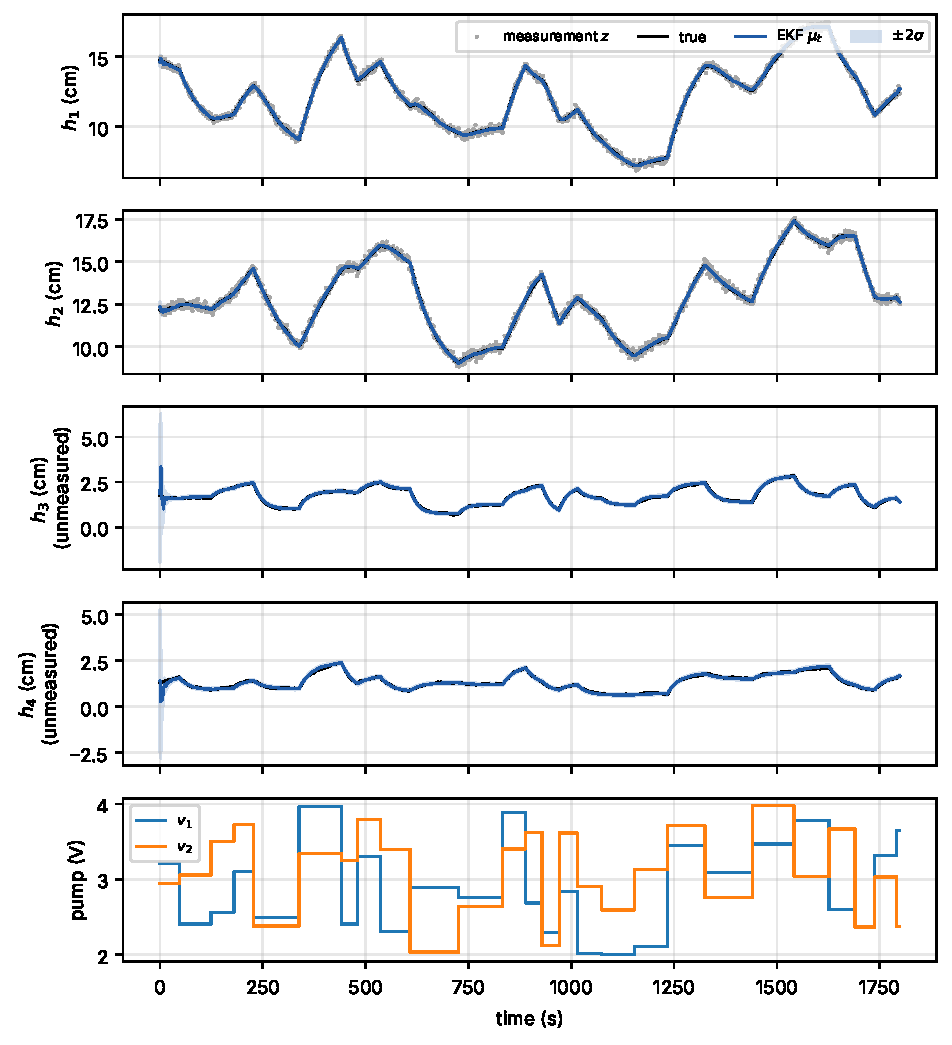
\includegraphics[width=0.95\linewidth]{figures/a1_tracking.pdf}
\caption{One test run. Grey dots: level measurements; black: true levels; blue: EKF mean with $\pm2\sigma$ band. $h_3$ and $h_4$ are never measured. Bottom: the random pump voltages.}\label{fig:track}
\end{figure}

\begin{table}[!htbp]
\centering\small
\caption{RMSE in cm over 50 Monte Carlo runs (200--1800\,s). ``Open loop'' runs the same discrete model from the same initial guess without measurement updates.}\label{tab:rmse}
\begin{tabular}{lcccc}\toprule
Estimator & $h_1$ & $h_2$ & $h_3$ (unmeasured) & $h_4$ (unmeasured)\\\midrule
Raw measurement $z_t$ & 0.150 & 0.151 & --- & --- \\
Open-loop model & 0.076 & 0.093 & 0.035 & 0.040\\
\textbf{EKF} & \textbf{0.038} & \textbf{0.038} & \textbf{0.034} & \textbf{0.038}\\\bottomrule
\end{tabular}
\end{table}

The EKF cuts the error on the measured levels by a factor of four relative to the raw sensors and by half relative to the model alone: it combines the two sources of information, as the Kalman gain intuition in the lectures suggests. For $h_3$ and $h_4$ the gain over the open-loop model is small. This is because the upper tanks are driven only by the (known) pump voltages and their own outflow, and the process noise in this setting is small, so the model alone already predicts them well. The measurements of $h_1$ and $h_2$ mainly help through the coupling $a_3\sqrt{2gh_3}$, which becomes important when the model is wrong (Section~\ref{sec:faults}).

\subsection{Consistency}
Figure~\ref{fig:cons} shows the average NEES and NIS over the 50 runs. With the true noise levels, ANEES $=4.10$ and ANIS $=2.01$, against expected values of 4 and 2. The averages lie inside the 95\,\% chi-square bands $[3.25,4.82]$ and $[1.48,2.59]$ for 95.3\,\% and 95.1\,\% of time steps, exactly what a consistent filter should show. The Euler discretisation and the linearisation therefore cause no measurable inconsistency at this noise level.

\begin{figure}[!htbp]
\centering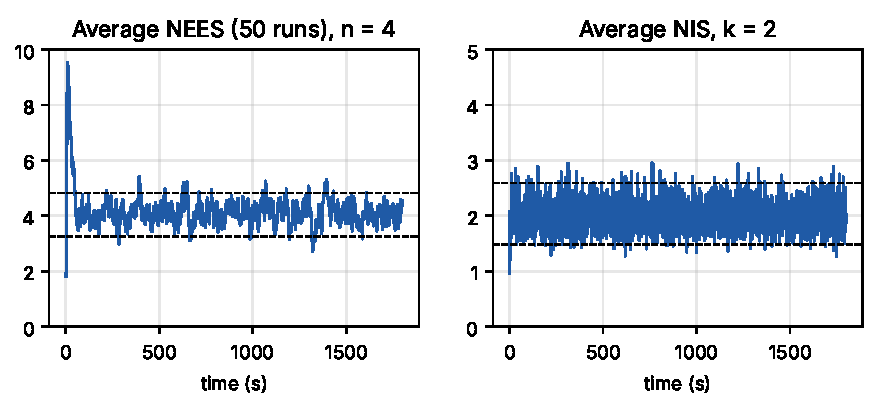
\includegraphics[width=0.95\linewidth]{figures/a2_consistency.pdf}
\caption{Average NEES (left) and NIS (right) over 50 runs with 95\,\% chi-square bands (dashed). The filter is consistent.}\label{fig:cons}
\end{figure}

\subsection{Sensitivity to the noise covariances}
In practice $R$ and $Q$ are not known and must be tuned. Figure~\ref{fig:sens} scales the assumed process-noise standard deviation from $0.25\times$ to $8\times$ its true value, for three settings of $Q$. Two effects are visible:
\begin{itemize}\itemsep0pt
\item \textbf{$R$ too small} (the model is trusted too much): the filter becomes \emph{overconfident}. ANEES rises to 13 at $0.5\times$ and 54 at $0.25\times$, and the RMSE also grows, because the filter ignores useful measurements.
\item \textbf{$R$ too large}: the filter is \emph{conservative} (ANEES $\approx1.3$) and noisier, since it follows the sensors too closely.
\end{itemize}
The RMSE is minimal, and ANEES $\approx4$, at the true value. Consistency tests therefore give a principled tuning target that does not require ground truth when NIS is used instead of NEES.

\begin{figure}[!htbp]
\centering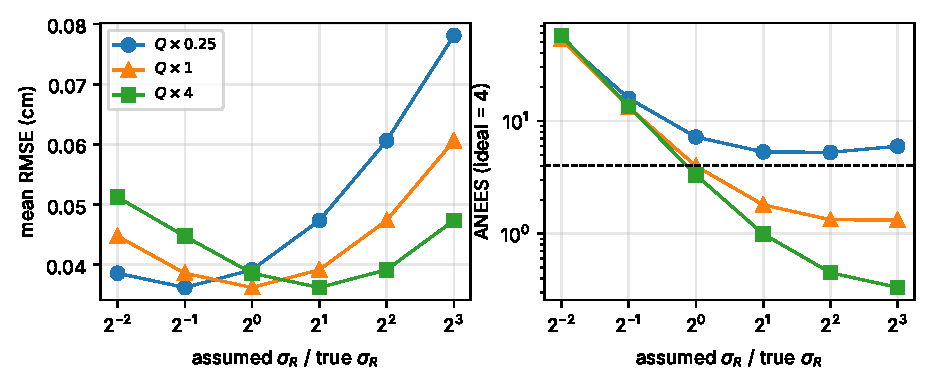
\includegraphics[width=0.95\linewidth]{figures/a3_sensitivity.pdf}
\caption{Effect of the assumed process noise (x-axis, relative to the truth) and measurement noise (lines) on accuracy (left) and consistency (right; ideal ANEES $=4$).}\label{fig:sens}
\end{figure}

\subsection{Sensor outage}
Figure~\ref{fig:drop} removes all measurements between 600 and 900\,s. The filter keeps predicting with the model (lines 1--2 only), and $\operatorname{tr}\Sigma_t$ grows from 0.0055 to 0.0167. The error stays inside the growing $\pm2\sigma$ band. The RMSE of $h_1$ during the outage is 0.105\,cm, still better than the raw sensor. When measurements return, the covariance collapses within a few seconds. This is the expected behaviour of a Bayesian filter: uncertainty grows honestly when information is missing.

\begin{figure}[!htbp]
\centering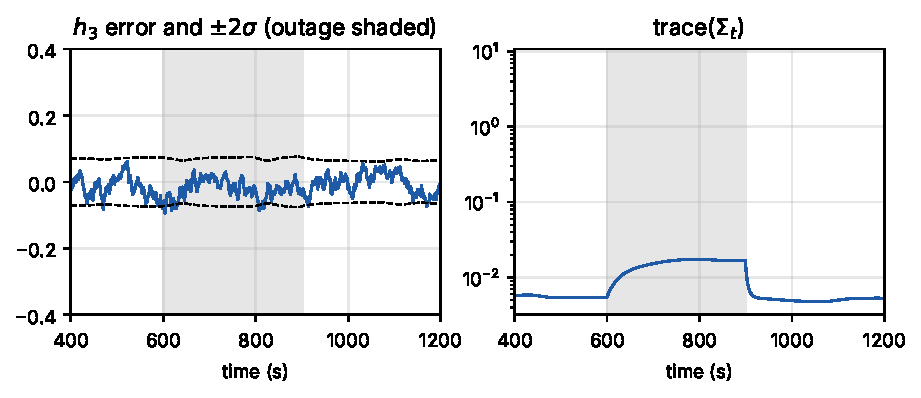
\includegraphics[width=0.95\linewidth]{figures/a4_dropout.pdf}
\caption{Sensor outage between 600 and 900\,s (shaded). Left: $h_3$ error and $\pm2\sigma$. Right: trace of the covariance.}\label{fig:drop}
\end{figure}

\subsection{Fault detection from the innovations}\label{sec:faults}
If the model is correct, NIS$_t\sim\chi^2_2$. I sum NIS over a sliding 30\,s window and raise an alarm when the sum exceeds a threshold. The threshold is set so that no more than 5\,\% of 20 separate fault-free runs raise any alarm. Two faults start at $t=900$\,s:
\begin{itemize}\itemsep0pt
\item a \textbf{leak in tank 3}: an extra outlet of 0.02\,cm$^2$. Tank 3 is \emph{unmeasured}, so the leak can only be seen through its effect on $h_1$;
\item a \textbf{sensor bias}: $+0.5$\,cm on sensor 1.
\end{itemize}
Over 30 runs, both faults were detected every time, with no false alarms before the fault. Median detection delays were \textbf{36\,s} for the leak and \textbf{5\,s} for the bias (Figure~\ref{fig:fault2}, left column). The two faults leave different signatures:
\begin{itemize}\itemsep0pt
\item \textbf{Leak:} NIS stays high, because the model keeps predicting more inflow to tank 1 than arrives.
\item \textbf{Bias:} NIS shows only a short spike. The filter soon ``explains'' the offset by shifting its estimate of $h_1$, so a persistent bias is partly absorbed. Detecting or estimating it reliably would need a bias state added to $x$, or a CUSUM test \cite{basseville1993}.
\end{itemize}

\section{Extension: EKF in the latent space of a learned world model}
The physics EKF needs an accurate model $g$. In many real systems no such model exists, but sensor logs with the applied control inputs do. Recent \emph{world models} learn the dynamics from such data. In particular, joint-embedding predictive architectures (JEPA) \cite{assran2023ijepa,assran2025vjepa2} learn to predict the \emph{representation} of the next observation rather than the raw observation. I tested whether the course EKF can be run inside such a learned model.

\subsection{Model}
The input $w_t$ is the last 20\,s of normalised $[z_t,u_t]$ (an 80-dimensional window). Three networks are used:
\begin{itemize}\itemsep0pt
\item an encoder $f_\theta$, a 2-layer tanh MLP, maps $w_t$ to a latent state $s_t\in\R^{12}$;
\item a target encoder $\bar f$ is an exponential moving average of $f_\theta$ \cite{grill2020byol};
\item an action-conditioned predictor implements the motion model in latent space:
\begin{equation}
p_\phi(s,u)=s+W_2^\top\tanh(W_1^\top[s;u]+b_1)+b_2 .
\end{equation}
\end{itemize}
Training minimises the 5-step latent prediction error $\|p_\phi^{k}(f_\theta(w_t),u_{t+1:t+k})-\bar f(w_{t+k})\|^2$, plus VICReg variance and covariance terms that prevent the latent space from collapsing \cite{bardes2022vicreg}. Nothing is reconstructed in sensor space. Because PyTorch was unavailable, I wrote a small reverse-mode autodiff engine for this (verified against finite differences). Training on 30 fault-free episodes (54\,000 samples) took about 35\,s on a laptop CPU.

\subsection{Latent EKF}
The latent state-space model used by the EKF is:
\begin{equation}
s_t=p_\phi(s_{t-1},u_t)+\varepsilon_t,\ \varepsilon_t\sim\mathcal N(0,R_{\text{lat}});\qquad y_t=\bar f(w_t)=s_t+\delta_t,\ \delta_t\sim\mathcal N(0,Q_{\text{lat}}).
\end{equation}
\begin{itemize}\itemsep0pt
\item \textbf{Motion model.} $g=p_\phi$, with an analytic Jacobian $G_t=I+W_2^\top\operatorname{diag}(1-a^2)W_{1,s}^\top$, where $a$ is the hidden activation.
\item \textbf{Measurement model.} JEPA has no decoder, so the target encoder's embedding of each new window is treated as a direct, noisy measurement of the latent state. This gives $h(s)=s$ and $H_t=I$.
\item \textbf{Noise covariances.} $Q_{\text{lat}}$ and $R_{\text{lat}}$ were estimated on validation runs from noise-free windows (only possible in simulation). A single scale factor (0.94) then matched the mean NIS to its expected value $d=12$.
\item \textbf{Read-out (evaluation only).} A small MLP maps latent states to the four levels.
\end{itemize}

\subsection{Results}
Table~\ref{tab:latent} and Figures~\ref{fig:lat}--\ref{fig:sweep} summarise the results.

\begin{table}[!htbp]
\centering\small
\caption{Estimation RMSE (cm, 30 test runs). ``Raw encoder'' reads the levels from $\bar f(w_t)$ without filtering.}\label{tab:latent}
\begin{tabular}{lcccc}\toprule
Estimator & $h_1$ & $h_2$ & $h_3$ & $h_4$\\\midrule
Raw encoder + read-out & 0.248 & 0.256 & 0.108 & 0.074\\
Latent EKF + read-out & 0.243 & 0.253 & 0.107 & 0.073\\
Physics EKF (reference) & 0.037 & 0.038 & 0.033 & 0.039\\\bottomrule
\end{tabular}
\end{table}

\begin{figure}[!htbp]
\centering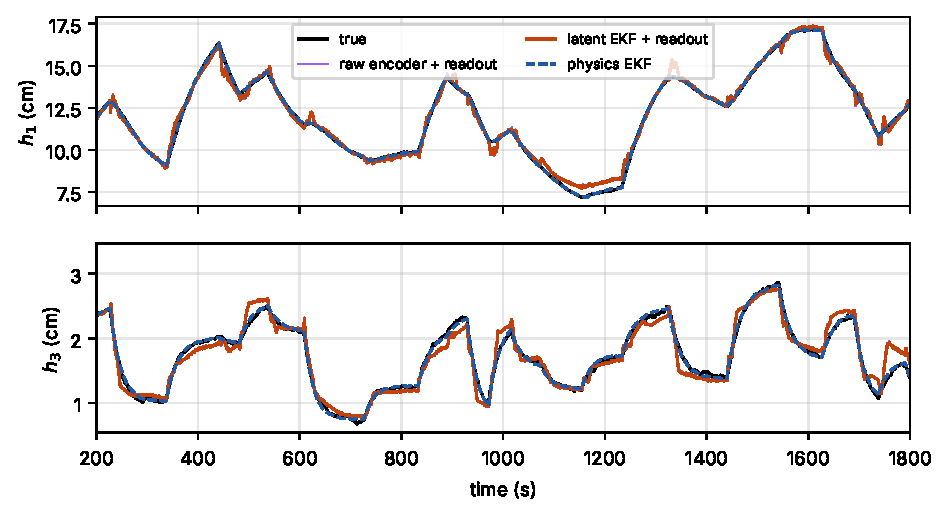
\includegraphics[width=0.95\linewidth]{figures/b3_latent_tracking.pdf}
\caption{Measured $h_1$ and unmeasured $h_3$ estimated without a physics model (latent EKF, orange) and with it (blue, dashed).}\label{fig:lat}
\end{figure}

\begin{figure}[!htbp]
\centering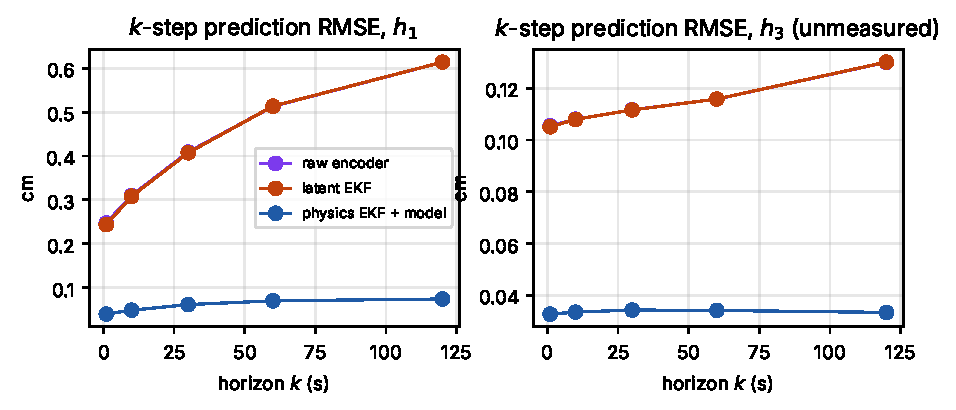
\includegraphics[width=0.95\linewidth]{figures/b2_prediction.pdf}
\caption{Open-loop $k$-step prediction error from the filtered state.}\label{fig:pred}
\end{figure}

\begin{figure}[!htbp]
\centering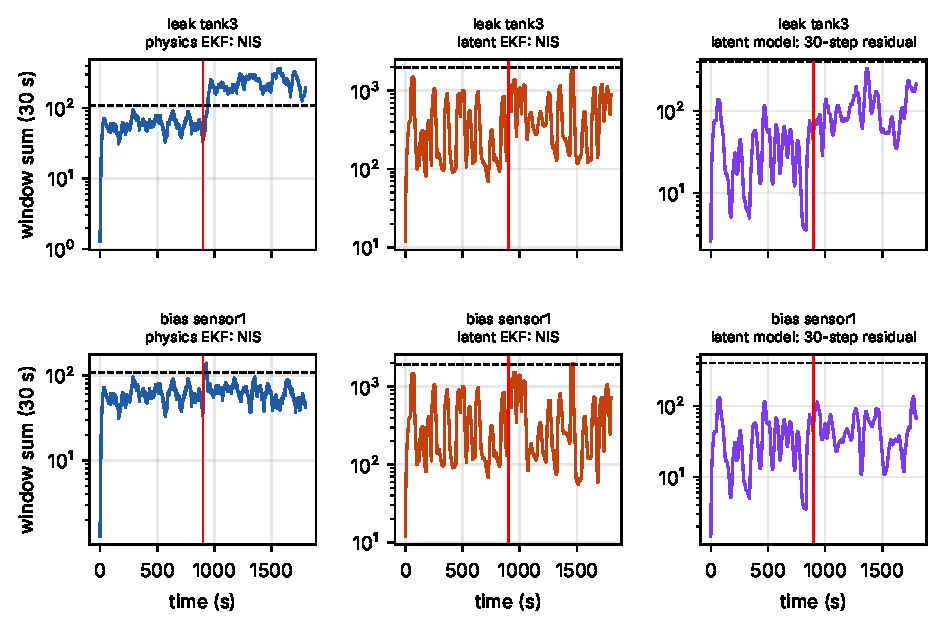
\includegraphics[width=\linewidth]{figures/b4_fault_detection.pdf}
\caption{Windowed fault statistics for one run of each fault (fault at the red line, threshold dashed). Physics NIS (left) responds clearly. The latent NIS (middle) is dominated by spikes at pump-voltage steps, where the learned predictor is least accurate.}\label{fig:fault2}
\end{figure}

\begin{figure}[!htbp]
\centering
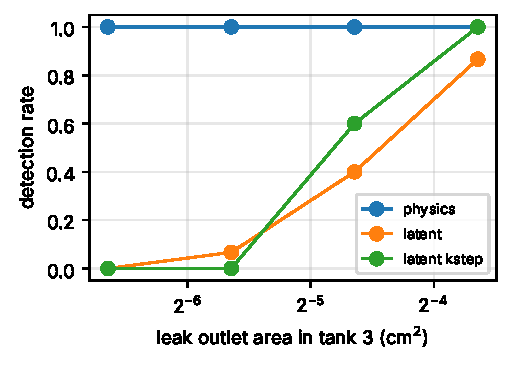
\includegraphics[width=0.48\linewidth]{figures/b5_leak_sweep.pdf}
\caption{Detection rate (15 runs per size) against leak size. The learned model only sees leaks two to four times larger than the one the physics EKF always detects.}\label{fig:sweep}
\end{figure}

\textbf{What worked.} With no physics knowledge, the learned model and latent EKF estimate the \emph{unmeasured} level $h_3$ to 0.11\,cm (3\,\% of its range). The latent NIS behaves like a calibrated $\chi^2_{12}$ statistic on fault-free data (mean 12.4).

\textbf{What did not, and why.} Three results fall short:
\begin{itemize}\itemsep0pt
\item \textbf{Little filtering gain.} The latent filter improves on the raw encoder by only about 2\,\%. The reason is visible in the noise estimates: $\operatorname{tr}R_{\text{lat}}=0.072$ while $\operatorname{tr}Q_{\text{lat}}=0.023$. The learned predictor's one-step error is three times larger than the latent measurement noise, so the Kalman gain is close to $I$ and the filter mostly follows the measurement. This is the same trade-off as in the $R$-sensitivity study: a filter can only add value when its model is more informative than its sensor.
\item \textbf{Prediction drift.} The learned model's prediction error grows with horizon much faster than the physics model's (Figure~\ref{fig:pred}).
\item \textbf{Weak fault detection.} For the 0.02\,cm$^2$ leak, the latent NIS detects 23\,\% of runs and a 30-step latent residual 3\,\%. The physics EKF detects 100\,\%. Both latent monitors reach 87--100\,\% for a 0.08\,cm$^2$ leak (Figure~\ref{fig:sweep}). The latent NIS spikes at every pump-voltage step (Figure~\ref{fig:fault2}). The predictor's error, and therefore the innovation, is not stationary, but $R_{\text{lat}}$ is a constant, so the chi-square threshold has to be set high to avoid false alarms.
\end{itemize}

\section{Discussion}
\textbf{The EKF works as theory predicts when its assumptions hold.} With an accurate model and correct $R$ and $Q$, it is consistent, uses the measurement coupling to estimate unmeasured states, degrades gracefully during outages, and its innovations give a sensitive fault monitor with a statistically defined threshold.

\textbf{Limitations of my implementation:}
\begin{enumerate}\itemsep0pt
\item \textbf{Linearisation.} It is accurate here because the levels stay away from zero. Near-empty tanks would make the $\sqrt h$ nonlinearity severe, and a UKF \cite{julier2004} or particle filter would be more appropriate.
\item \textbf{Simulation only.} The noise is Gaussian and white, and the true covariances are known; real sensors need $R$ and $Q$ identified, for example from the innovations \cite{mehra1970}.
\item \textbf{The latent EKF breaks two EKF assumptions.} First, consecutive latent measurements come from overlapping windows, so their noise is correlated (lag-1 autocorrelation 0.27). Second, the model error depends on the input, so a constant $R_{\text{lat}}$ is wrong.
\end{enumerate}

\textbf{How this project will continue.} The extension shows that ``Kalman filtering in a learned latent space'' is feasible but that the learned model's uncertainty, not the filter, is the bottleneck. I will continue it as a research project with four aims: (i) predict an input-dependent $R_{\text{lat}}(s,u)$ so that the latent NIS stays calibrated through transients; (ii) estimate $R_{\text{lat}}$ and $Q_{\text{lat}}$ online from the innovations instead of from simulation; (iii) use the calibrated innovation test as a run-time ``can I trust my world model?'' monitor and compare it with established fault-detection methods on the Tennessee Eastman benchmark and real plant data; and (iv) use the filtered latent belief for model-predictive control. Related approaches include KVAE \cite{fraccaro2017kvae} and KalmanNet \cite{revach2022kalmannet}; neither is decoder-free with an innovation-based trust monitor.

\section{Conclusion}
I implemented the Extended Kalman filter from the course derivation for the nonlinear quadruple-tank process and verified it with Monte Carlo accuracy and chi-square consistency tests. With the physics model, the EKF estimates all four levels to below 0.04\,cm from two noisy sensors, stays consistent (ANEES 4.10 versus 4), handles a 300\,s outage, and detects a hidden tank leak and a sensor bias within 36\,s and 5\,s. Running the same EKF in the latent space of a learned JEPA world model recovers the unmeasured levels without any physics, but reveals that the learned model's error dominates. Calibrating that uncertainty is what makes the innovation test useful, and it is the direction I will pursue next.

\begin{thebibliography}{99}\small
\bibitem{thrun2005} S.~Thrun, W.~Burgard, D.~Fox, \emph{Probabilistic Robotics}. MIT Press, 2005.
\bibitem{kalman1960} R.~E.~Kalman, ``A new approach to linear filtering and prediction problems,'' \emph{J. Basic Engineering}, 82(1):35--45, 1960.
\bibitem{johansson2000} K.~H.~Johansson, ``The quadruple-tank process: a multivariable laboratory process with an adjustable zero,'' \emph{IEEE Trans. Control Systems Technology}, 8(3):456--465, 2000.
\bibitem{barshalom2001} Y.~Bar-Shalom, X.~R.~Li, T.~Kirubarajan, \emph{Estimation with Applications to Tracking and Navigation: Theory, Algorithms and Software}. Wiley, 2001.
\bibitem{mehra1970} R.~K.~Mehra, ``On the identification of variances and adaptive Kalman filtering,'' \emph{IEEE Trans. Automatic Control}, 15(2):175--184, 1970.
\bibitem{willsky1976} A.~S.~Willsky, ``A survey of design methods for failure detection in dynamic systems,'' \emph{Automatica}, 12(6):601--611, 1976.
\bibitem{basseville1993} M.~Basseville, I.~V.~Nikiforov, \emph{Detection of Abrupt Changes: Theory and Application}. Prentice Hall, 1993.
\bibitem{julier2004} S.~J.~Julier, J.~K.~Uhlmann, ``Unscented filtering and nonlinear estimation,'' \emph{Proc. IEEE}, 92(3):401--422, 2004.
\bibitem{assran2023ijepa} M.~Assran et al., ``Self-supervised learning from images with a joint-embedding predictive architecture,'' \emph{CVPR}, 2023.
\bibitem{assran2025vjepa2} M.~Assran et al., ``V-JEPA 2: Self-supervised video models enable understanding, prediction and planning,'' arXiv:2506.09985, 2025.
\bibitem{grill2020byol} J.-B.~Grill et al., ``Bootstrap your own latent: a new approach to self-supervised learning,'' \emph{NeurIPS}, 2020.
\bibitem{bardes2022vicreg} A.~Bardes, J.~Ponce, Y.~LeCun, ``VICReg: Variance-invariance-covariance regularization for self-supervised learning,'' \emph{ICLR}, 2022.
\bibitem{fraccaro2017kvae} M.~Fraccaro, S.~Kamronn, U.~Paquet, O.~Winther, ``A disentangled recognition and nonlinear dynamics model for unsupervised learning,'' \emph{NIPS}, 2017.
\bibitem{revach2022kalmannet} G.~Revach et al., ``KalmanNet: neural network aided Kalman filtering for partially known dynamics,'' \emph{IEEE Trans. Signal Processing}, 70:1532--1547, 2022.
\end{thebibliography}

\end{document}
